\section{Durchf"uhrung}
	\label{sec:durchfuehrung}

		Bei den Versuchen war besonders darauf zu achten, dass je eine Platte der X- und Y- Ablenkung geerdet sein sollte. 
		Anschlie"send musste die Stromversorgung etwa $\SI{1}{\minute}$ anheizen, bevor der Kippschalter von "`Standby"' auf "`On"' gestellt werden durfte.
		Nun ist die gew"unschte Be\-schleu\-ni\-gungs\-span\-nun\-g angelegt worden.
		Die nun auf dem Leuchtschirm erschienene Abbildung des Elektronesstrahls wurde nun mit Hilfe der Fokussierungspannung wurde so geregelt, dass ein m"oglichst kleiner Leuchtfleck zu sehen ist.
		Dabei war darauf zu achten, dass der Elektronenstrahl nicht allzulange auf der selben Position des Schirms bleibt, da dieser ansonsten besch"adigt wird.

		\subsection{Versuch 501}
		\label{sub:501}

		\begin{figure}[h]
			\centering
			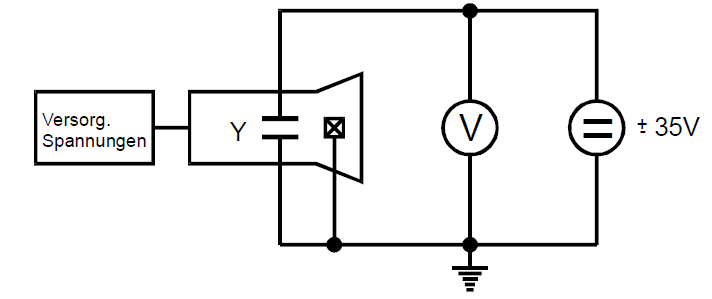
\includegraphics[width = 14cm]{img/501a.png}
			\caption{Schaltung zur Messung der Leuchtfleckbestimmung in Abh"angigkeit von der Ablenkspannung}
			\label{501a}
		\end{figure}

		Der Versuch wurde gem"a"s Abbildung \ref{501a} aufgebaut, um die Proportionalit"at zwischen der Leuchtfleckverschiebung $D$ und der Ablenkspannung $U_d$ f"ur $5$ verschiedenen Be\-schleu\-ni\-gungs\-span\-nun\-gen $U_B$ zu "uberpr"ufen. 
		Dazu sollte $U_d$ bei jeder Messreihe so eingestellt werden, dass der Leuchtfleck auf die $9$ "aquidistanten Linien des Koordinatennetzes trifft.
		$U_d$ wurde bei jeder Messung auf dem Voltmeter abgelesen.

		\begin{figure}[h]
			\centering
			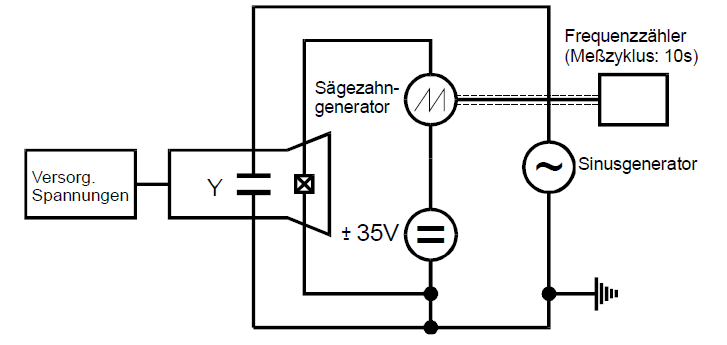
\includegraphics[width = 14cm]{img/501b.png}
			\caption{Prinzipschaltung eines Kathodenstrahl Oszillographen}
			\label{501b}
		\end{figure}

		Im $2.$ Versuchsteil sollte ein einfacher Kathodenstrahl-Oszillograph nach Abbildung \ref{501b} gebaut werden.
		Nun wurde versucht durch Ver"anderung der S"agezahnfrequenz $\nu_{s"a}$ stehende Bilder der Sinusspannung auf dem Leuchtschirm zu erzeugen.
		Dazu muss die S"agezahn- und die Sinusfrequenz ein rationales Verh"altnis bilden. In diesem Fall sollten die Situationen f"ur $n\nu_{s"a} = \nu_{si}; n = \frac{1}{2}, 1, 2, 3 $ eingestellt werden und die S"agezahnfrequenz $\nu_{s"a}$ am Fre\-quenz\-z"ah\-ler ablesen werden.
		$U_B$ wurde konstant gehalten und die Maximale Strahlauslenkung in Y-Richtung gemessen.

	\subsection{Versuch 502} 
	\label{sub:502}
		
		Bei diesem Versuch wurde zus"atzlich ein homogenes Magnetfeld erzeugt, dessen Richtung senkrecht zum Elektronenstrahl der Elektronenstrahlr"ohre steht. Dies war mit Hilfe einer Helmholtz-Spule m"oglich, dessen Helmholtz-Feld $B_{HF}$ im Mittelpunkt gegeben ist durch

		\begin{eqnarray*}
			B = \mu_0 \frac{8}{\sqrt{125}} \frac{NI}{R}
		\end{eqnarray*}
		{\centering
		(N = Windungszahl, I = Spulenstrom, R = Spulenradius, $\mu_0 = 4\pi*10^{-7}$)\\
		}
		\vspace{0.3 cm}    
		Im ersten Versuchsteil musste die Elektronenstrahlr"ohrevor Beginn in Richtung der Horizontalkomponente des Erdmagnetfeldes ausgerichtet werden, welche mithilfe des Deklinatorium-Inklinatoriums auffindbar war. Nun wurde bei zwei konstanten Be\-schleu\-ni\-gungs\-span\-nun\-gen Messungen der Strahlverschiebung $D$ in Abh"angigkeit von $B_{HF}$ durchgef"uhrt. Dazu wurde der Leuchtfleck bei $B_{HF} = 0$ auf die oberste oder unterste Linie des Koordinatenetzes mit einem elektrischen Feld verschoben.\\
		\newline
		Im n"achsten Versuchsteil wurde der Versuchsaufbau in Nord-S"ud-Richtung ausgerichtet und der Leuchtfleck bei m"oglichst niedriger Be\-schleu\-ni\-gungs\-span\-nun\-g in den Nullpunkt des XY-Koordinatennetzes gelegt.
		Nun wurde der Versuchsaufbau in Ost-West Richtung ausgerichtet und die Auslenkung durch das Erdmagnetfeld mit Hilfe des Helmholtz-Feldes kompensiert. Wenn der Leuchtfleck nach dem Einstellen eines geeigneten Spu\-len\-stroms $I_{hor}$ wieder im Ursprung liegt gilt $B_{HF} = -B_{hor}$ des Erdmagnetfeldes.\\
		\newline
		Abschlie"send wurde der Inklinationswinkel $\varphi$ zur Bestimmung der Totalintensit"at $B_{total}$ gemessen.
		Dazu wurde das Inklinatorium um die vertikale Achse gedreht, sodass die Magnetnadel parallel zur horizontalen Drehachse des Ger"ates liegt.
		Anschlie"send schwenkt man den Teilkreis um $\SI{90}{^\circ}$. Nun zeigt die Magnetnadel genau in Feldrichtung und $\varphi$ kann abgelesen werden.